\documentclass[t]{beamer}

% Load general definitions
% Preamble file - general definitions, package loading, etc.

%=================================
% Load packages
\usepackage{amssymb,amsmath}
\usepackage{graphicx}
\usepackage{url}
\usepackage{tikz}
\usetikzlibrary{mindmap,trees,arrows}
\usepackage{fancyvrb}
\usepackage[portuguese]{babel} 
\usepackage[utf8]{inputenc}
\usepackage{subfigure}
\usepackage{times}
\usepackage[T1]{fontenc}
\usepackage{cancel}
\usepackage{color}
\usepackage{listings}
\usepackage[document]{ragged2e}
\usepackage{physics}
\usepackage{amsmath}
\usepackage{tikz}
\usepackage{mathdots}
\usepackage{yhmath}
\usepackage{cancel}
\usepackage{color}
\usepackage{siunitx}
\usepackage{array}
\usepackage{multirow}
\usepackage{amssymb}
\usepackage{gensymb}
\usepackage{tabularx}
\usepackage{extarrows}
\usepackage{booktabs}
\usetikzlibrary{fadings}
\usetikzlibrary{patterns}
\usetikzlibrary{shadows.blur}
\usetikzlibrary{shapes}

%=================================
% Set mode
\mode<presentation>
{
	\usetheme{Madrid}
	\usecolortheme{structure}
	\useoutertheme{infolines}
	\setbeamercovered{invisible}
}

% Get rid of nav bar
\beamertemplatenavigationsymbolsempty

% Insert frame number at bottom of the page.
\usefoottemplate{\hfil\tiny{\color{black!90}\insertframenumber}} 

%=================================
% Define new commands

\newcommand\Real{{\mathbb{R}}}
%\newcommand{\vi}{\vspace{0.6\baselineskip}}
%\newcommand{\goodgap}{\hspace{\subfigtopskip}\hspace{\subfigbottomskip}}


% Equation environments
\newcommand{\beq}{\begin{equation}}
\newcommand{\eq}{\end{equation}}
\newcommand{\beqs}{\begin{equation*}}
\newcommand{\eqs}{\end{equation*}}
\newcommand{\beqn}{\begin{eqnarray}}
\newcommand{\eqn}{\end{eqnarray}}
% Bold variables
\newcommand{\mbf}[1]{\ensuremath{\mathbf{#1}}}
% Itemization
\newcommand{\bitem}{\begin{itemize}}
\newcommand{\eitem}{\end{itemize}}
\newcommand{\spitem}{\vskip 1em\item}
\newcommand{\bitems}{\begin{itemize}\item}
\newcommand{\benums}{\begin{enumerate}\item}
\newcommand{\eenum}{\end{enumerate}}
% color blocks
\newenvironment{colorblock}[2]{%
\setbeamercolor{block title}{#2}
\begin{block}{#1}}{\end{block}}
% Vertical spacing
\newcommand{\vone}{\vskip 1em}
\newcommand{\vhalf}{\vskip .5em}
% Frame environments
\newenvironment{ftst}[3][t]{%
\begin{frame}{environment=ftst,#1}
\frametitle{#2}
\framesubtitle{#3}}{\end{frame}}
\newenvironment{ftstf}[2]{
\begin{frame}[fragile,environment=ftstf]
\frametitle{#1}
\framesubtitle{#2}}{\end{frame}}
% colors
\definecolor{MyGray}{rgb}{0.5,0.5,0.5}
\definecolor{MyDBGray}{rgb}{0.1,0.1,0.4}
\definecolor{darkgreen}{rgb}{0,0.4,0}
\definecolor{black}{rgb}{0,0,0}
\def\defn#1{{\color{red} #1}}
% Footnote
\renewcommand{\thefootnote}{\alph{footnote}}
% Relaxed footnotes
\newcommand{\lfr}[1]{\let\thefootnote\relax\footnote{\tiny #1}}
% Verbatim environment - using FANCYVRB package
\DefineVerbatimEnvironment%
{rcode}{Verbatim}
{fontsize=\scriptsize}
% Verbatim environment - using LISTINGS package
%\lstnewenvironment{rcode} {\lstset{	language = R,
%									basicstyle = \scriptsize\ttfamily,
%									showspaces = false,
%									showstringspaces = false,
%									showtabs = false,
%									keywordstyle = \color{black}\bfseries,
%									commentstyle = \color{darkgreen},
%									numbers = none,
%									otherkeywords={	<-,
%													ggplot,
%													geom_boxplot,
%													facet_grid,
%													shapiro.test,
%													fligner.test,
%													glht,
%													with},
%									deletekeywords={data,
%													model,
%													residuals,
%													c,
%													axis,
%													default,
%													labels,
%													qq.text}}}%
%{}

% Specific definitions
\title[]{Banco de dados II}
\subtitle[]{Escalonamento de Transações}
\author[]{Patrícia Lucas\\{\footnotesize }}
\institute{Bacharelado em Sistemas de Informação \\ IFNMG  - Campus Salinas}
\date{\scriptsize Salinas\\Março 2022}

\begin{document}

% cover page
\setbeamertemplate{footline}{}
\begin{frame}

\begin{center}
\includegraphics[width=.15\textwidth]{}
\end{center}
  \titlepage
  \begin{tikzpicture}[remember picture,overlay]
  \node[anchor=south east,xshift=-5pt,yshift=5pt] at (current page.south east) {\tiny Versão 1.2021};
  \node[anchor=south west,yshift=0pt] at (current page.south west) {
\includegraphics[width=.25\textwidth]{Logos/salinas_horizontal_jpg.jpg}};
  \end{tikzpicture}  
\end{frame}

% Main slides

\begin{ftst}{Referência}{Escalonamento de Transações}
\begin{figure}
    \centering
    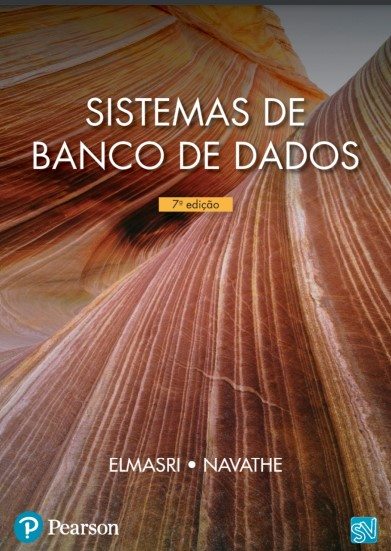
\includegraphics[scale=0.4]{Figuras/book.jpg}
\end{figure}
ELMASRI, R.; NAVATHE, S. B. Sistemas de Banco de Dados. 7. ed. São Paulo: Pearson Addison Wesley, 2019.
\end{ftst}

%==================================

\begin{ftst}{Conceito}{Escalonamento de Transações}

\begin{itemize}
    \item \textbf{Escalonamento} é uma sequência de instruções que especificam a ordem cronológica na qual as instruções de transações simultâneas são executadas.
    \item Um escalonamento para um conjunto de transações deve consistir em todas as instruções dessas transações.
    \item Deve preservar a ordem em que as instruções aparecem em cada transação individual.
\end{itemize}
\end{ftst}

%==================================

\begin{ftst}{Conceito}{Escalonamento de Transações}

\begin{itemize}
    \item Uma transação que conclui com sucesso sua execução terá uma instrução COMMIT como sua última operação. O COMMIT garante que os efeitos da transação serão registrados no BD mesmo que ocorra uma falha.
    \item Uma transação que não consegue concluir sua execução deverá ter uma instrução ABORT como sua última operação. O ABORT solicita ao SGBD que desfaça as operações.
    \item Notação simplificada para escalonamento:
    \begin{itemize}
        \item $r_i(X)$: read_item(X) na transação $T_i$.
        \item $w_i(X)$: write_item(X) na transação $T_i$.
        \item $c_i$: commit na transação $T_i$.
        \item $a_i$: abort na transação $T_i$.
    \end{itemize}
\end{itemize}
\end{ftst}

%==================================

\begin{ftst}{Conceito}{Escalonamento de Transações}

\begin{itemize}
    \item Exemplos de escalonamento:
    \begin{itemize}
        \item $S_a: r_1(X); r_2(X); w_1(X); r_1(Y); w_2(X); w_1(Y); c_1; c_2$.
        \item $S_b: r_1(X); w_1(X); r_2(X); w_2(X); r_1(Y); a_1; c_2$.
    \end{itemize}
\end{itemize}
\begin{figure}
    \centering
    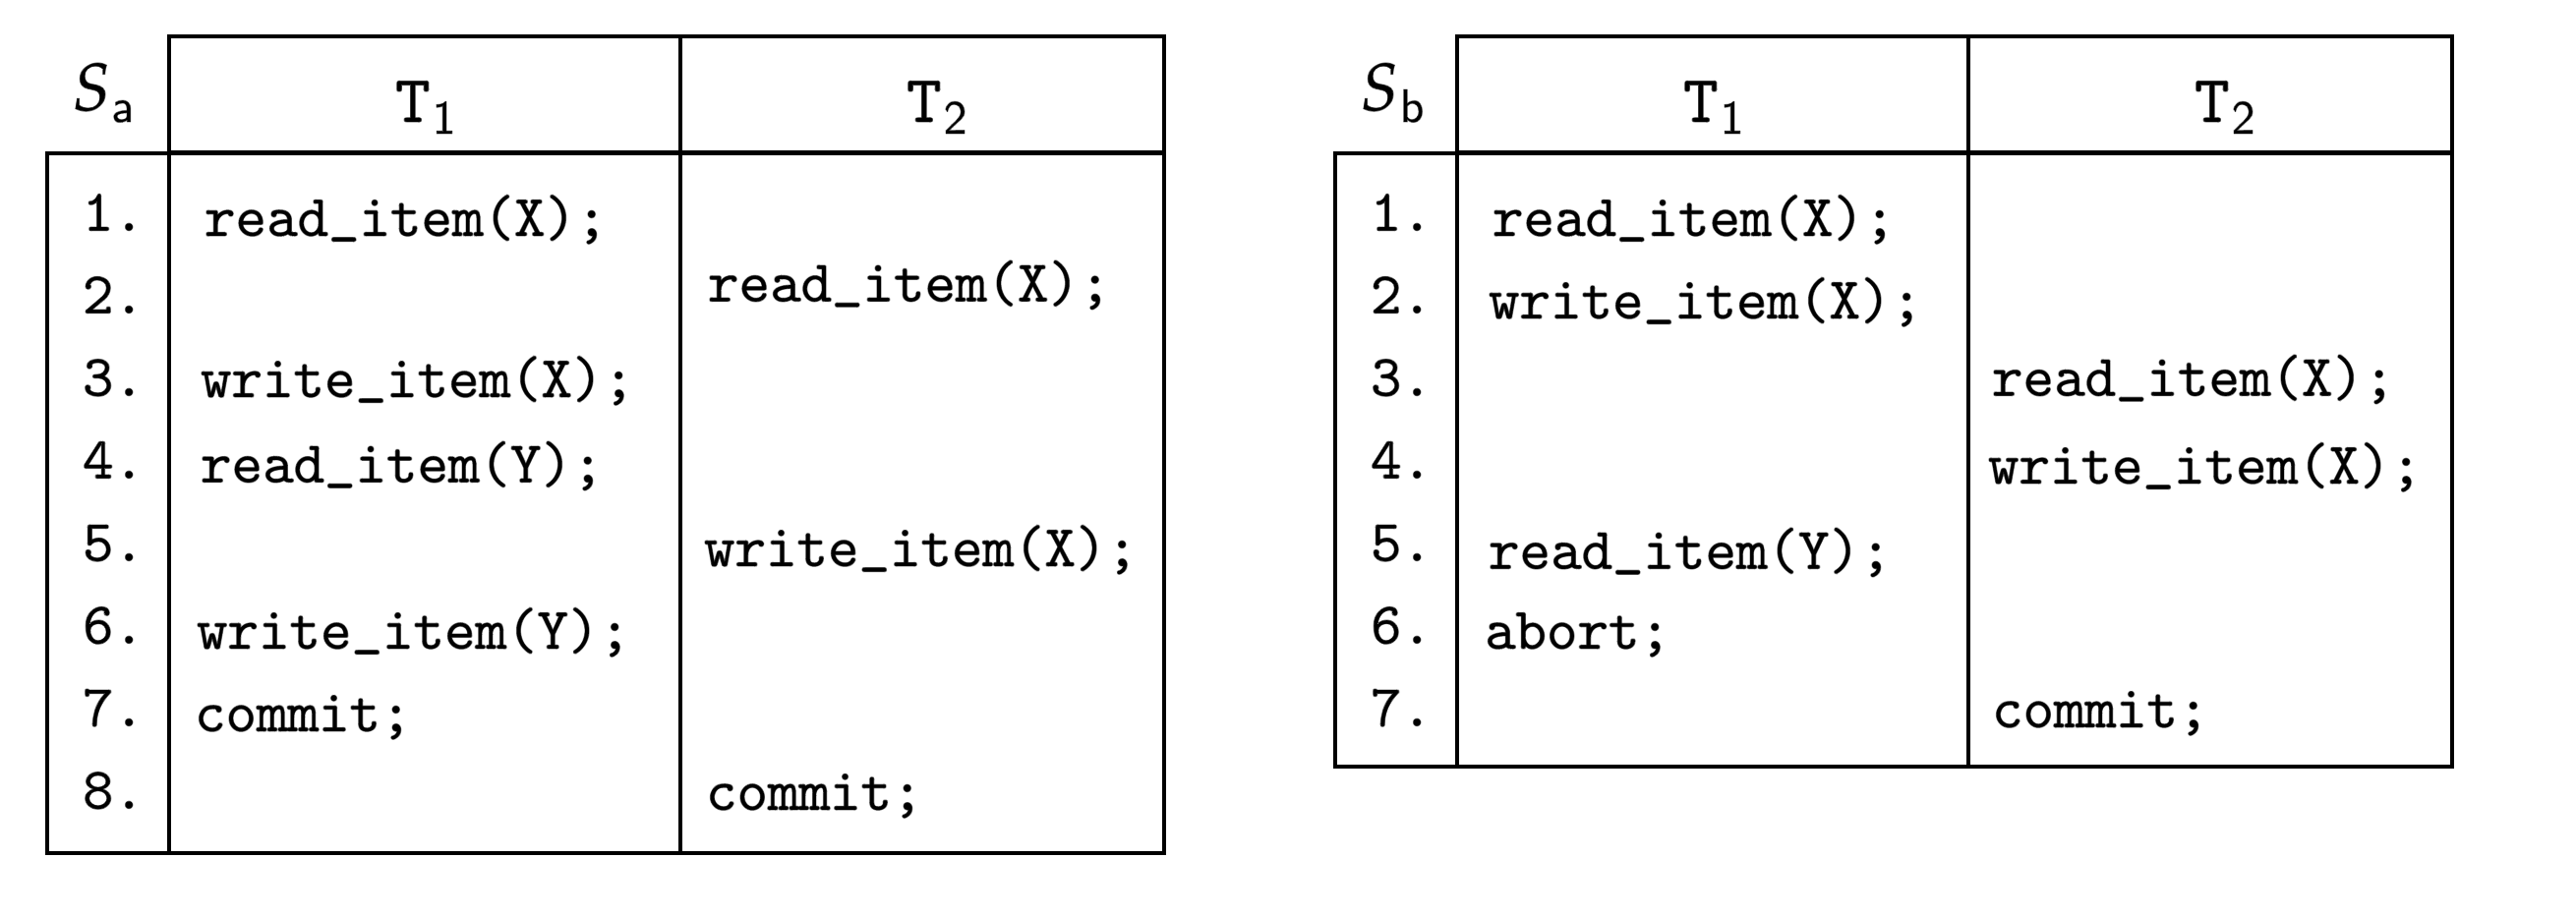
\includegraphics[scale=0.13]{Figuras_transacoes/11.png}
\end{figure}
\end{ftst}

%==================================

\begin{ftst}{Escalonamento Serial}{Escalonamento de Transações}

\begin{itemize}
    \item Exemplo de escalonamento serial onde $T_1$ é seguida por $T_2$.
\end{itemize}
\begin{figure}
    \centering
    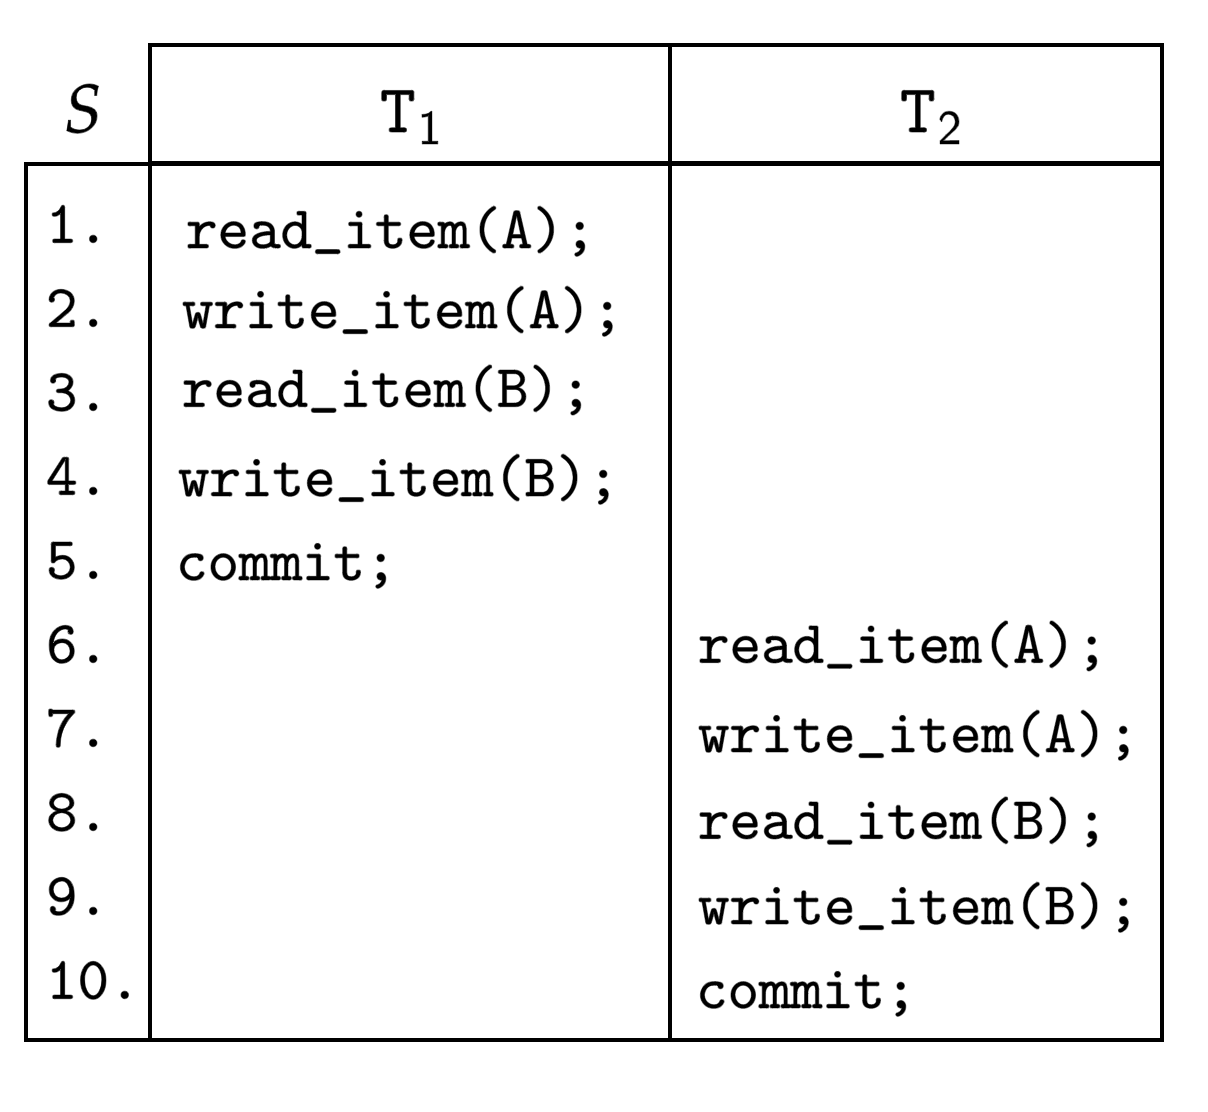
\includegraphics[scale=0.15]{Figuras_transacoes/12.png}
\end{figure}
\end{ftst}

%==================================

\begin{ftst}{Escalonamento Serial}{Escalonamento de Transações}

\begin{itemize}
    \item Exemplo de escalonamento serial onde $T_2$ é seguida por $T_1$.
\end{itemize}
\begin{figure}
    \centering
    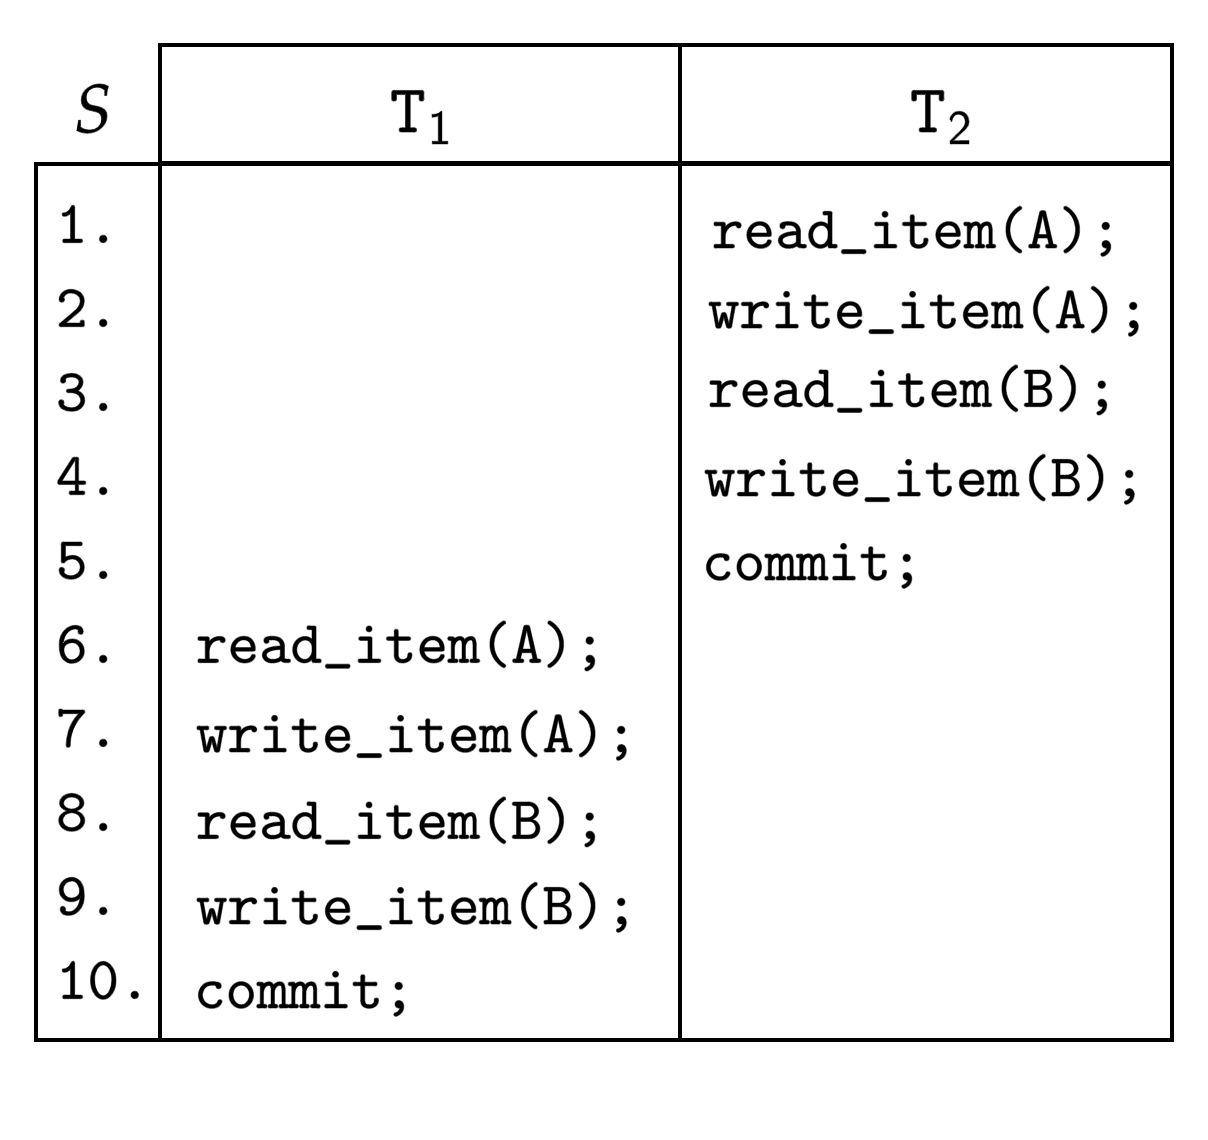
\includegraphics[scale=0.14]{Figuras_transacoes/13.png}
\end{figure}
\small
\begin{itemize}
    \item Qual a vantagem do escalonamento serial? E qual a desvantagem?
\end{itemize}
\end{ftst}

%==================================

\begin{ftst}{Escalonamento não-serial}{Escalonamento de Transações}

\begin{itemize}
    \item Exemplo:
\end{itemize}
\begin{figure}
    \centering
    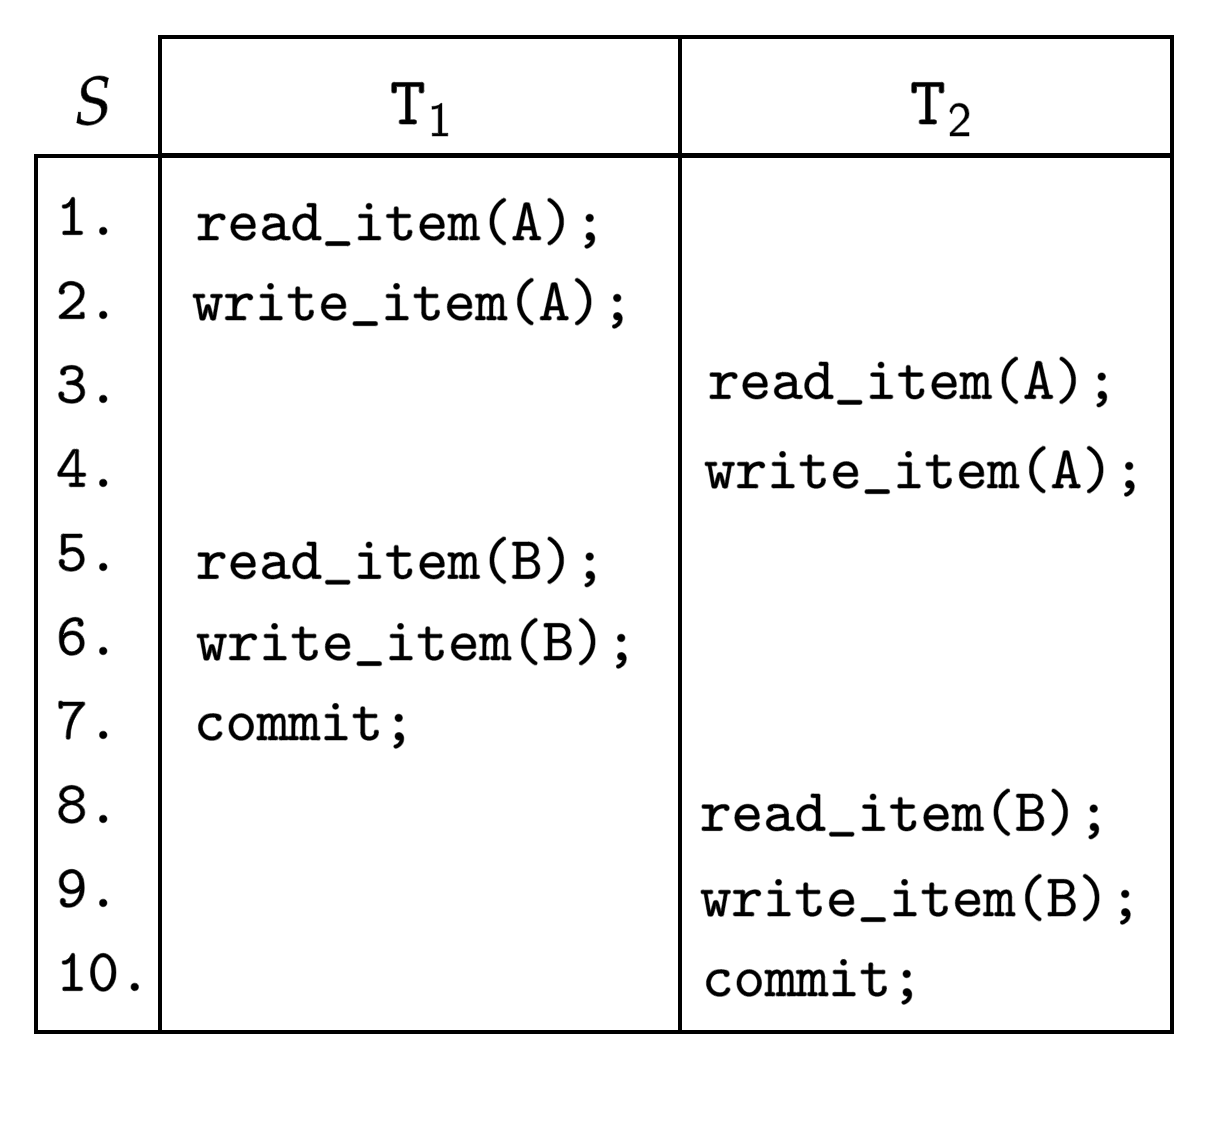
\includegraphics[scale=0.12]{Figuras_transacoes/14.png}
\end{figure}
\small
\begin{itemize}
    \item Qual a vantagem do escalonamento não-serial?
    \item Esse escalonamento possui as mesmas operações que os escalonamentos seriais anteriores, porém explora a concorrência.
\end{itemize}
\end{ftst}

%==================================

\begin{ftst}{Seriabilidade}{Escalonamento de Transações}

\begin{itemize}
    \item Cada transação preserva individualmente a consistência do BD.
    \item Assim, a execução \textbf{serial} de um conjunto de transações preserva a consistência do BD.
    \item Um escalonamento é \textbf{serializável} se for equivalente a um escalonamento serial.
    \item Formas de equivalência:
    \begin{itemize}
        \item Seriabilidade por conflito.
        \item Seriabilidade por visão.
    \end{itemize}
\end{itemize}

\end{ftst}

%==================================

\begin{ftst}{Seriabilidade}{Escalonamento de Transações}
\textbf{Instruções Conflitantes}
\vone
\begin{itemize}
    \item Sejam $I_i$ e $I_j$ duas instruções das transações $T_i$ e $T_j$, respectivamente.
    \item Elas são conflitantes se, e somente se, houver algum item de dados $Q$ acessado por $I_i$ e $I_j$, e pelo menos uma dessas instruções escreveu em $Q$.
\end{itemize}

\begin{table}[]
\centering
\begin{tabular}{|c|c|c|}
\hline
\textbf{$I_i$} & \textbf{$I_j$} & \textbf{Conflito} \\ \hline
read\_item(Q)  & read\_item(Q)  & Não               \\ \hline
read\_item(Q)  & write\_item(Q) & Sim               \\ \hline
write\_item(Q) & read\_item(Q)  & Sim               \\ \hline
write\_item(Q) & write\_item(Q) & Sim               \\ \hline
\end{tabular}
\end{table}

\end{ftst}

%==================================

\begin{ftst}{Seriabilidade}{Escalonamento de Transações}

\textbf{Instruções Conflitantes}
\vone
\begin{itemize}
    \item Exemplo: quais operações são conflitantes no escalonamento $S_a$ e $S_b$?
    \vone
    \item $S_a: r_1(X); r_2(X); w_1(X); r_1(Y); w_2(X); w_1(Y); c_1; c_2$.
    \vone
    \item $S_b: r_1(X); w_1(X); r_2(X); w_2(X); r_1(Y); a_1; c_2$.

\end{itemize}


\end{ftst}

%==================================

\begin{ftst}{Seriabilidade}{Escalonamento de Transações}
\textbf{Instruções Conflitantes}
\vone
\begin{itemize}
    \item Um conflito entre $I_i$ e $I_j$ força uma ordem temporal entre elas.
    \item Se $I_i$ e $I_j$ forem consecutivas, mas não conflitantes, a ordem temporal em que elas ocorrem no escalonamento pode ser alterada.

\end{itemize}

\end{ftst}

%==================================

\begin{ftst}{Seriabilidade por conflito}{Escalonamento de Transações}

\begin{itemize}
    \item Se um escalonamento $S$ pode ser transformado em um escalonamento $S'$ por uma série de trocas de ordem de instruções não-conflitantes, dizemos que $S$ e $S'$ são \textbf{equivalentes por conflito}.
    \item Dizemos que um escalonamento $S$ é \textbf{serializável por conflito} se for \textbf{equivalente por conflito} a um escalonamento \textbf{serial}.

\end{itemize}

\end{ftst}

%==================================

\begin{ftst}{Seriabilidade por conflito}{Escalonamento de Transações}
\textbf{Exemplo:} os escalonamentos $S_a$ e $S_b$ são equivalentes por conflito?

\begin{figure}
    \centering
    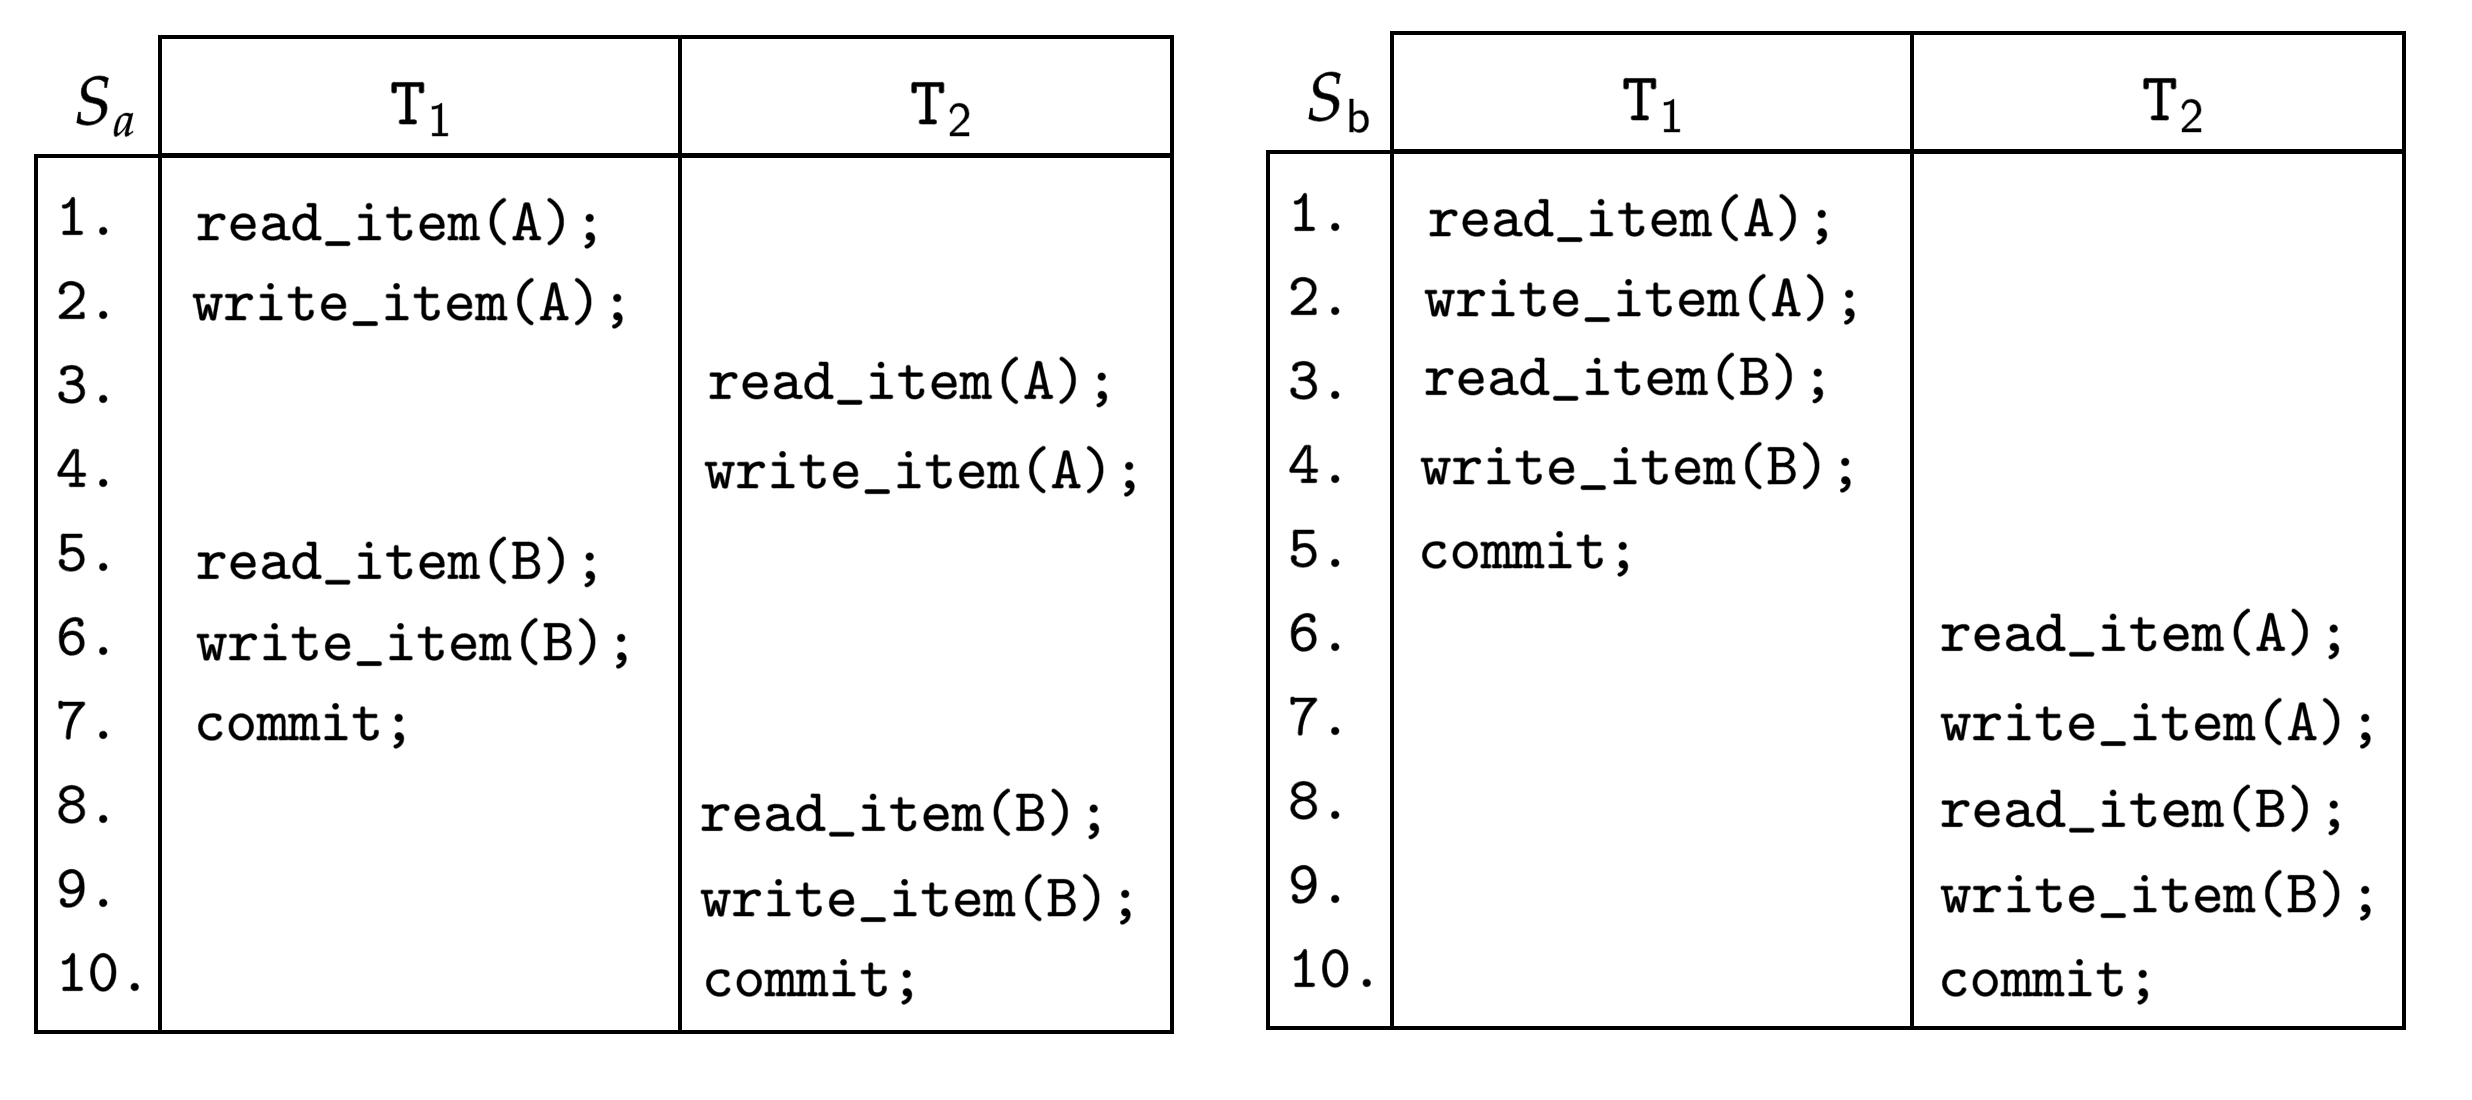
\includegraphics[scale=0.13]{Figuras_transacoes/15.png}
\end{figure}

\end{ftst}




\end{document}